%%
% SigLog paper on HoTT
% May 2014
% IHP
%%
\documentclass[11pt]{article}
\usepackage{amsmath}
\usepackage{amssymb,latexsym}
\usepackage{amsthm}
\usepackage{bm}
\input{prooftree}
\usepackage[all,cmtip]{xy}
\input{diagxy}
\CompileMatrices       
\usepackage{url}
\usepackage{tikz}
\usepackage{pdfpages}

\usepackage[color=green!40]{todonotes}



% categories
\newcommand{\C}{\ensuremath{\mathbb{C}}}
\newcommand{\B}{\ensuremath{\mathbb{B}}}
\newcommand{\N}{\ensuremath{\mathbb{N}}}
\newcommand{\T}{\ensuremath{\mathbb{T}}}
\newcommand{\CC}{\ensuremath{\mathcal{C}}}
\newcommand{\BB}{\ensuremath{\mathcal{B}}}
%\newcommand{\EE}{\ensuremath{\mathcal{E}}}
\newcommand{\psh}[1]{\ensuremath{\mathsf{Set}^{#1^{\mathrm{op}}}}}
\newcommand{\Set}{\ensuremath{\mathsf{Set}}}
\newcommand{\Cat}{\ensuremath{\mathsf{Cat}}}
\newcommand{\covpsh}[1]{\ensuremath{\mathsf{Set}^{#1}}}
%\renewcommand{\to}{\ensuremath{\rightarrow}}
\newcommand{\pocorner}[1][dr]{\save*!/#1+1.2pc/#1:(1,-1)@^{|-}\restore}
\newcommand{\pbcorner}[1][dr]{\save*!/#1-1.2pc/#1:(-1,1)@^{|-}\restore}
\newcommand{\y}{\ensuremath{\mathsf{y}}} % Yoneda embedding

% arrows
\newcommand{\hook}{\ensuremath{\hookrightarrow}}
\newcommand{\mono}{\ensuremath{\rightarrowtail}}
%\newcommand{\epi}{\ensuremath{\twoheadrightarrow}}


% cubical sets
\newcommand{\I}{\ensuremath{\mathrm{I}}}
\renewcommand{\H}{\ensuremath{\mathbb{H}}}
\newcommand{\HH}{\ensuremath{\mathcal{H}}}

% type theory
\newcommand{\G}{\ensuremath{\Gamma}}
\newcommand{\defeq}{=_{\mathrm{def}}}
\newcommand{\type}{\mathsf{type}}       
\newcommand{\types}[2]{#1 \vdash #2:\type}
\newcommand{\Gtypes}[1]{\types{\Gamma}{#1}}
\newcommand{\term}[2]{#1\,:\,#2}
\newcommand{\terms}[2]{#1 \vdash #2}
\newcommand{\Gterms}[1]{\terms{\Gamma}{#1}}
\newcommand{\ext}[2]{{#1\!\centerdot\! #2}}
\newcommand{\ty}{\ensuremath{\,:\,}}
\newcommand{\pair}[1]{\ensuremath{\langle #1\rangle}}
\newcommand{\exdot}{\ensuremath{\!\centerdot\!}}
\newcommand{\texdot}{\ensuremath{\centerdot}}

% Id types
\newcommand{\Id}{\mathsf{Id}}
\newcommand{\id}[1]{\Id_{#1}}
\newcommand{\refl}{\mathsf{refl}}
\newcommand{\rec}{\mathsf{rec}}
\newcommand{\idrec}{\mathsf{idrec}}
\newcommand{\jay}{\mathsf{j}}
\renewcommand{\i}{\mathsf{i}}

% Universe
\newcommand{\U}{\ensuremath{\mathcal{U}}}
\newcommand{\UU}{\ensuremath{\widetilde{\mathcal{U}}}}

% theorem styles
\newtheorem{theorem}{Theorem}
\newtheorem*{theorem*}{Theorem}
\newtheorem{proposition}[theorem]{Proposition} 
\newtheorem{lemma}[theorem]{Lemma}
\newtheorem{corollary}[theorem]{Corollary} 

\theoremstyle{remark}
\newtheorem{remark}[theorem]{Remark} 
\newtheorem*{remarks*}{Remarks}
\newtheorem{example}[theorem]{Example}

\theoremstyle{definition}
\newtheorem{definition}[theorem]{Definition}

%%%%%%%%%%%%%%%%%%%%%%%%%%%%%%%%%%%%%%%%%%%%%%%%%%%%
\begin{document}
%%%%%%%%%%%%%%%%%%%%%%%%%%%%%%%%%%%%%%%%%%%%%%%%%%%%

\title{Some title}
\author{Steve Awodey \and Robert Harper}
\date{\today}

\maketitle
%%%%%%%%%%%%%%%%%%%%%%%%%%%%%%%%%%%%%%%%%%%%%%%%%%%%

\todo[inline]{Are we promoting ``Univalent Foundation'' or ``Homotopy Type Theory''?  Is it ``Homotopy Type Theory'' or
  ``Higher-Dimensional Type Theory''?}

Homotopy Type Theory is an emerging currently emerging unification of previously disparate frameworks for formalizing
and mechanizing mathematics, one based on a computational conception of the type of a construction, the other based on a
homotopical conception of the (homotopy) type of a space.  Indeed, the name ``homotopy type theory'' can be read in two
ways, as ``(homotopy type) theory'' and ``homotopy (type theory)'', neatly summarizing the consolidation of ideas at the
heart of the subject.  The computational notion of type has its origins in Brouwer's program of intuitionism, which
sought to ground mathematics in the concept of an effective construction (one would say ``algorithm'' these days).  The
homotopical notion of type emerges from abstract homotopy theory, in particular Grothendieck's conception of a space as
an $\infty$-groupoid.  The former perspective was developed most fully by Per Martin-L\"{o}f, leading in particular to
his Intuitionistic Theory of Types, on which Homotopy Type Theory is based.  The latter was initiated by Awodey and
Warren, who first observed that the so-called ``identity type'' of Martin-L\"{o}f's Type Theory has the structure of an
$\infty$-groupoid, and can be interpreted in any Quillen Model Category, a framework for doing abstract homotopy theory.
The connection was clinched by Voevodsky's formulation of the \emph{univalence axiom}, which, roughly speaking, relates
the homotopy-theoretic concept of equivalence to that of the aforementioned identity type.

Because univalence plays such a central role, Voevodsky has suggested that the unification of the computational and
homotopical perspectives be called the \emph{Univalent Unification} of two major lines of development in mathematics.  A
critically important point is that the univalent unification is \emph{fully compatible} with classical mathematics; it
does not involve any principles that are incompatible with classical reasoning, though it does, at the outset, avoid
postulating axioms that are unnecessary for much of the development.  Indeed, the Homotopy Type Theory contains within
it the whole of ZF set theory, with or without the Axion of Choice, and with or without the Law of the Excluded Middle,
two principles that lie at the heart of classical mathematics and that have, regrettably, been obstacles to the kind of
unification described here.  But by not insisting on these axioms globally, it is possible to consider a far richer
notion of type than has hitherto been possible in the computational setting, namely one in which types are abstract
spaces that have non-trivial higher-dimensional structure, as exemplified by familiar examples such as the $n$-spheres
for all $n\geq 0$.  Rather than being ``coded up'' as certain sets living within certain conceptions of space, such as a
topological space, these objects arise \emph{synthetically} within the theory, characterized by their introductory and
eliminatory forms (mapping-in and mapping-out properties, or universal properties), rather than by how they are
constructed as sets.  This perspective greatly simplifies well-known constructions, such as the Hopf fibration or the
Eilenberg-MacLane spaces, and supports remarkably simple and clear proofs of well-known results such as the
classification of the fundamental groups of the spheres.

What is it that makes the univalent unification possible?  Although it may be too early to formulate a deep unifying
principle, it is possible to make a few observations that will give the reader a sense of its inevitability.  First, all
of the constructions of Intuitionistic Type Theory, including especially the previously enigmatic identity type, are
homotopy invariant, meaning that type families and mappings between types inherently respect ``paths'' in space
representing \emph{identifications} of points in the space.  In particular the formation of type-indexed products and
sums of types correspond to analogous constructions on spaces, and, most importantly, the identity type, take as a
whole, corresponds to the \emph{total path space} of a space, as originally observed by Awodey and Warren.  Second, a
characteristic feature of both intuitionistic type theory and higher homotopy theory is the emphasis on \emph{structure}
over \emph{property}.  In intuitionistic mathematics types express propositions, and objects of the type are proofs of
those propositions in the form of mathematical constructions that provide evidence for their truth.  A similar emphasis
is found in abstract homotopy theory, in which paths (homotopies) may be seen as evidence for the identification (in a
sense, ``equality'') of two points.  Two points are not merely equal as a property, but rather are identified by a
particular construction.  This approach extends to higher dimensions in that one may speak of the identification of two
(parallel) identifications, at all higher dimensions.  Such structure is found in standard settings such as simplicial
sets, cubical sets, and globular sets, all of which stress the role of cells as identifications, with the Kan condition
ensuring that this interpretation validates the higher groupoid laws and that families and maps respect homotopy.

The culmination of this line of thought is the univalence axiom, which governs paths in a Grothendieck universe, a type
whose elements are themselves types and which is closed under the standard type-formation operations, but for the
formation of the universe itself.  The question arises as to what is the appropriate notion of identification for
elements of the universe?  Voevodsky's crucial observation is that two types in a so-called univalent universe ought to
be identified whenever they are homotopy equivalent, precisely because all of the constructions of type theory, which
are internalized by the universe, are homotopy invariant.  This is essentially an application of Leibniz's Principle
stating that two things are equal if they cannot be distinguished, but extended to the (proof-relevant) concept of
identification, rather than merely (proof-irrelevant) equality.  On these grounds univalence is intuitively plausible,
but it has also been mathematically justified in two ways, by Voevodsky's (classical) model in simplicial sets, and
Bezem, \textit{et al.}'s (constructive) model in cubical sets.  Developing the computational content of homotopy type
theory remains an active area of investigation that promises to influence computing practice much as the intuitionistic
version has done.

*******************

This is not the place for a systematic introduction (for that, see \cite{HoTTbook}), or even a general survey (such as \cite{apw,pw}), but a brief example may serve to convey a bit of the flavor of the new approach, especially the distinctive intermingling of logical and homotopical ideas.  As is the case in conventional Martin-L\"of type theory, the basic types of booleans $\B$ and natural numbers $\N$ can have at most one identification between any two elements; that is, given say $n, m : \N$ and $p,q: \id{\N}(n,m)$ we always have $\alpha:\id{\id{\N}(n,m)}(p,q)$.  In this sense, there is no real information in the types $\id{\N}(n,m)$ apart from whether or not they are inhabited.  Such types with at most one identification between any two elements are called (``homotopy 0-types'' or simply) ``sets''.  Any types that can be constructed from $\B$, $\N$, or any other sets, by means of the usual type constructors of dependent sum $(\Sigma{x:A})B(x)$ and dependent product $(\Pi{x:A})B(x)$ (which includes $A\times B$ and $A\rightarrow B$ as special cases) are also sets, and the same is true for the equality types $\id{A}(a,a')$ for $a,a':A$, for any set $A$.  

 An example of a type that is not a set is the circle (or ``$1$-sphere'') $S^1$, which has a base point $b: S^1$ with many different self-identifications $\refl(b),\, p,\, p\cdot p,\, ... :\id{S^1}(b,b)$.  Here $\refl(b)$ is the trivial identification, i.e.\ the canonical witness to the reflexivity of identity, but there is also another identification $p$ which is different from $\refl(b)$ in the sense that $\id{\id{S^1}(b,b)}(\refl(b), p)$ is empty.  We can think of $p$ homotopically as the continuous ``path" that goes once around the circle. 

%
% draw a circle here, with b and p indicated"
%
By the (function witnessing the) transitivity of equality, 
\[
(-)\cdot(-) : \id{S^1}(a,b) \times \id{S^1}(b,c)\to \id{S^1}(a,c),
\]
 there are also the ``paths'' $p\cdot p,\, p\cdot p\cdot p,\, \ldots$.   And by symmetry,
 \[
 (-)^{-1}:\id{S^1}(a,b) \to \id{S^1}(b,a),
 \]
 there are similarly the paths $p^{-1},\, p^{-1}\cdot p^{-1}, \ldots :\id{S^1}(b,b)$.  Although $S^1$ is therefore not a set, it can be shown that $\id{S^1}(b,b)$ is one; that is, the types $\id{\id{S^1}(b,b)}(x,y)$ are either inhabited (by reflexivities) or empty, depending on whether or not $x=y$, for all $x,y : \id{S^1}(b,b)$ --- we say that $S^1$ is a ``(homotopy) 1-type".  This fact follows from the specification of $S^1$ as a new kind of \emph{higher} inductive type, generalizing the usual specification of the natural numbers and similar structures.  For $S^1$, the inductive specification essentially says that it is the type freely generated by the base point $b:S^1$ and the loop $p:\id{S^1}(b,b)$, in the same sense that the usual inductive specification of $\N$ says that it is the type freely generated by $0:\N$ and the successor function $s:\N\to\N$.  
  
 Another type that is not a set is the universe $\U$ of all (small) types.  According to the new Univalence Axiom, identifications between types $A,B:\U$ correspond to ``equivalences" $A\simeq B$, which are generalized type isomorphisms.  In fact, if $A$ and $B$ themselves are sets, then an equivalence between them is just an isomorphism in the usual sense: a pair of maps back and forth that compose to the respective identity mapppings.  Now the booleans $\B$, for example, have two different isomorphisms $\B\simeq \B$, namely the identity and the operation of ``negation'' $\neg:\B\to\B$, which swaps the truth values $0,1:\B$.  Thus by univalence there are two distinct identifications in $\id{\U}(\B,\B)$, corresponding to these distinct isomorphisms, and so $\U$ is not a set, but, like $S^1$, a ``higher-dimensional" type.  
 
Now observe that by the basic recursive property of $S^1$ as ``the type freely generated by a point and a loop on it'', there is a map $$\rec(\B,n): S^1 \to \U$$ determined by sending the base point $b:S^1$ to the booleans $\B:\U$ and the generating loop $p : \id{S^1}(b,b)$ to (the loop corresponding under univalence to) negation, say $n : \id{\U}(\B,\B)$.  As a type of the form $\B\to\U$, this $\rec(\B,n)$ is thus a family of types over $\B$, sometimes called a ``dependent type" and written $x:\B \vdash \rec(\B,n)(x)$.  Homotopically, such a type-family is interpreted as a ``fibration" $E\to\B$, where the total space $E$ is just the sum type $(\Sigma{x:\B})\rec(\B,n)(x)$, equipped with its usual indexing projection.  In the present case, the ``fiber" is then the type $\rec(\B,n)(b) = \B$, and the action on (elements of) $\B$ induced by the path $n: \id{S^1}(b,b)$ in the base is exactly the operation of negation $\neg : \B\to \B$.  Thus, from a homotopical point of view, we have constructed the ``twisted double cover'' of the circle (see figure \ref{fig:winding}).
 % fix this:
\begin{figure}\centering
  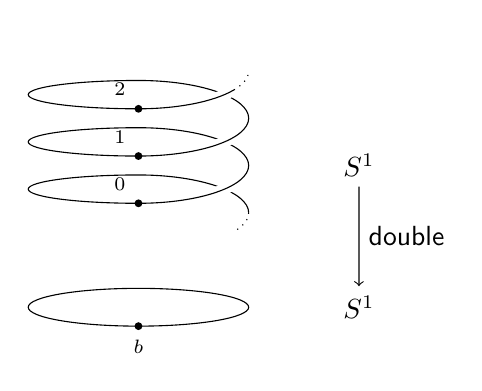
\begin{tikzpicture}[xscale=1.4,yscale=.6]
    \node (R) at (2,1) {$S^1$};
    \node (S1) at (2,-2) {$S^1$};
    \draw[->] (R) -- node[auto] {$\mathsf{double}$} (S1);
    \draw (0,-2) ellipse (1 and .4);
    \draw[dotted] (1,0) arc (0:-30:1 and .8);
    \draw (1,0) arc (0:90:1 and .8) arc (90:270:1 and .3) coordinate (t1);
    \draw[white,line width=4pt] (t1) arc (-90:90:1 and .8);
    \draw (t1) arc (-90:90:1 and .8) arc (90:270:1 and .3) coordinate (t2);
    \draw[white,line width=4pt] (t2) arc (-90:90:1 and .8);
    \draw (t2) arc (-90:90:1 and .8) arc (90:270:1 and .3) coordinate (t3);
    \draw[white,line width=4pt] (t3) arc (-90:90:1 and .8);
    \draw (t3) arc (-90:-30:1 and .8) coordinate (t4);
    \draw[dotted] (t4) arc (-30:0:1 and .8);
    \node[fill,circle,inner sep=1pt,label={below:\scriptsize $b$}] at (0,-2.4) {};
    \node[fill,circle,inner sep=1pt,label={above left:\scriptsize 0}] at (0,.2) {};
    \node[fill,circle,inner sep=1pt,label={above left:\scriptsize 1}] at (0,1.2) {};
    \node[fill,circle,inner sep=1pt,label={above left:\scriptsize 2}] at (0,2.2) {};
  \end{tikzpicture}
  \caption{The twisted double cover of $S^1$ in classical topology}\label{fig:winding}
\end{figure}
%
This important construction from homotopy theory is closely related to the famous Hopf fibration used to compute some higher homotopy groups of the spheres $S^2$ and $S^3$.  Indeed, one can also construct the Hopf fibration in much the same way, using univalence, negation, winding around the circle, and other constructions derived from combinations of logical, type-theoretic, and homotopical ideas.  

This sort of reasoning gives an entirely new ``synthetic" approach to classical mathematics, which not only allows for the explicit logical formalization of classical results like the calculations of homotopy groups of spheres, but also permits their formal verification in computational proof systems based on a constructive system of logic.

*********************

one important point about the univalent framework is that is subsumes both the classical set-theoretic framework for doing mathematics, and it is "almost" subsumes the constructive framework.  as to the former, we need only explain the hierarchy of n-types, and the fact that classical proof-irrelevant propositions are -1-types, and that classical sets are 0-types (wherein equality of sets is taken as "self-evident"), and that these levels are compatible with lem and with ac as usually conceived, so that standard zfc-based math slots right it without difficulty.  but the advantage of univalent foundations is that it provides infinitely much more structure than just that, and it is fascinating and useful to explore the mathematics of higher n-types, and the uses of proof-relevance at higher dimensions.  as to the latter, the main issue is that the constructive framework, while also by design compatible with classical mathematics (by virtue of being limited to 0-types and -1-types), has a computational foundation---truth is explained in terms of running programs.  this fact has been the central driving force in research in pl's, semantics, and verification for the last several decades, and is clearly of paramount importance.  so the question becomes, can we achieve a grand unification of computational types and homotopy types that provides the richness of hlevels and the foundational and practical pleasures of being justified solely on the basis of computation?  we can say that we are tantalizingly close to achieving such a unification, perhaps via the cubical sets interpretation recently proposed, perhaps through other means currently under investigation.

Some more things to mention:

- formal verification of mathematics as a practical tool makes logical foundations finally relevant to mathematical practice, rather than just a theoretical possibility.  In fact, if the latter is their only interest, then Goedel matters, but given the actual practical benefits, Goedel doesn't. This is a new "post-Goedel" attitude to logical foundations. 

- can something similar be said about foundations of computation ?  did people ever worry about Goedel the way the logicians do in connection with foundations of math?

- higher category theory turns out to be naturally described by constructive methods, while the subsystem of 0-categories (i.e. the sets) still admits classical logic, without forcing the higher dimensional part to also be classical.  This seems to be a new way of conceiving of the relation between classical and constructive methods -- not as distinct systems related to each other as "stronger versus weaker", or even as the different  logic of "constant versus variable" objects, but as compatible subsystems of a single system that are simultaneously applicable to different parts of the universe, distinguished by the intrinsic complexity or "dimension" of the objects therein.

we can close with saying that we are on the cusp of a revolution, in which two self-contained, well-motivated, well-justified, yet completely disparate frameworks for doing mathematics are not only being consolidated into a single, well-motivated, well-justified framework, but moreover the unified theory enriches and extends the classical framework without disrupting anything that has been achieved in that setting?

%%%%%%%%%%%%%%%%%%%%%%%%%%%%%%%%%%%%%%%%%%%%%%%%%%%%
\begin{thebibliography}{300}
%%%%%%%%%%%%%%%%%%%%%%%%%%%%%%%%%%%%%%%%%%%%%%%%%%%%

\bibitem{AW}
S.~Awodey and M.A.~Warren. Homotopy theoretic models of identity types. \emph{Math. Proc. Camb. Phil. Soc.}, 146, 45--55, 2009.

\bibitem{GvdB}
B.~van den Berg and R.~Garner. Topological and Simplicial Models of Identity Types. \emph{ACM Transactions on Computational Logic}, 13:1, 2012.

\bibitem{CwF} 
P.~Dybjer. ``Internal Type Theory." \emph{LNCS} 1158, 120--134, 1996.

\bibitem{HS} Hofman and Streicher 

\bibitem{HoTTbook} 
\emph{Homotopy Type Theory: Univalent Foundations of Mathematics}, The Univalent Foundations Program, Institute for Advanced Study, 2013. {\tt http://homotopytypetheory.org/book}

\bibitem{KLV}  
C.~Kapulkin, P.~LeFanu Lumsdaine and V.~Voevodsky, The Simplicial Model of Univalent Foundations. \emph{In preparation}, 2013.

%
\end{thebibliography}

%%%%%%%%%%%%%%%%%%%%%%%%%%%%%%%%%%%%%%%%%%%%%%%%%%%%
\end{document}
%%%%%%%%%%%%%%%%%%%%%%%%%%%%%%%%%%%%%%%%%%%%%%%%%%%%
